\section{Cross-Layer Analysis\\Methodology}\label{sec:qxdmresults}

We use QxDM to perform cross-layer analysis for several purposes.  In \S\ref{sec:exp.setup} we describe how we collect ground truth data transmission information in the IP and RLC layers.  We describe the cross-layer mapping algorithm in \S\ref{sec:cross.layer.algo} that allows us to understand the impact of RLC-layer behavior on higher layers, and in \S\ref{sec:rlc.retx.cal} we describe how we calculate the RLC retransmission ratio in QxDM.

%\S\ref{sec:verify.latency} verifies the latency observations using cross layer algorithm.
%\S\ref{sec:ctrl.exp} illustrates the control experiments for further the root cause identification. 

\subsection{QxDM Experiments}\label{sec:exp.setup}

% Describe what the tool does
QxDM is a real-time data collection and diagnostic logging tool for measuring \textit{Radio Frequency} (RF) performance in mobile devices~\cite{qxdm_flyer}. It allows us to gain insight into lower layer RLC transmission information.  
\TReport{It is a Windows based monitoring application. When I perform control experiments and real application measurements, I plug in the device to the desktop or laptop with QxDM software installed. }
The tool was used to collect data on IP packets, RLC data PDUs, and RRC states, as well as RLC control PDUs and RLC configuration information such as polling timers and retransmission limits.  \Paperonly{The experiments performed were done on two devices from two different manufacturers, which we will call M1 and M2.  The M1 device runs Android OS 4.1.1, and the M2 device runs Android OS 4.0.4. This allows us to study potential device-dependent behavior.}

 %We plan to extend this analysis to more device types.
\begin{TReports}
Once the experiments finished, we filtered out the real-time monitoring information related to IP packets, RLC PDUs (protocol data unit, the smallest data transmission unit in RLC layer), and RRC states in Table~\ref{tab:QxDM.logs}, and dumped the results into a log file. The 0x11EB log entry includes IP headers, IP payloads, and its customized header. Since large IP packets will be fragmented into smaller segments, the customer header could indicate the segment index of the whole IP packet. The 0x4132 and 0x4133 unveil the RLC AM (acknowledge mode) configurations, i.e. the polling function timers, the retransmission limit for a single PDU, and etc. The 0x413B, and 0x418B provides RLC PDU header and first byte payload information for both data PDUs and control PDUs (or STATUS PDUs) in both uplink and downlink directions. We wrote a QxDM log parser to aggregate the filtered entries, and apply cross layer analysis to understand the correlation between different layers. We conducted all the experiments on two devices -- Galaxy S3 with Android OS 4.1.1 and HTC One S with Android OS 4.0.4, to observe any device dependent behavior.


QxDM provides precise RRC state information to indicate the current radio channel state. RLC data PDU and status PDU will assist us in cross layer mapping to the transport layer data, i.e. TCP/UDP. Other context information could also be found in the log, i.e. signal strength and physical layer transmission bit rate. The QxDM log is essentially a list of log entries formatted as a uniformed header with timestamp, a detailed log entry description, and a raw hex dump result.  

 Table of QxDM entries
\begin{table}[t!]
\begin{tabularx}{0.5\textwidth}{ | c | X | }
	\hline
  	\textbf{QxDM Log ID} & \textbf{Description} \\
  	\hline\hline
  	0x11EB & IP data packets \\
  	\hline
  	0x4132 & WCDMA RLC downlink acknowledge mode configuration \\
  	\hline
  	0x4133 & WCDMA RLC uplink acknowledge mode configuration \\
  	\hline
  	0x413B & WCDMA RLC uplink acknowledge mode PDU \\
  	\hline
  	0x418B & WCDMA Flexible RLC downlink acknowledge mode PDU \\
  	\hline
  	0x4125 & WCDMA RRC states \\
  	\hline
\end{tabularx}
\ncaption{QxDM log entries used in cross layer analysis}
\label{tab:QxDM.logs}
\end{table}
\end{TReports}

%\subsection{QxDM Experiments}\label{sec:ctrl.exp}

% UDP/ TCP control experiment set up

%\mycomment{To validate our proposed RRC state inference methodology,... Need to say how to validate this}
First, we validate the RRC inference methodology discussed above. We calculate the RRC demotion timers directly from QxDM logs.  According to the 3GPP spec~\cite{spec-3G-RRC}, the sender receives a \textit{radio bearer reconfiguration} (RBR) message from the Node B (\textit{i.e.} the base station) when it demotes from DCH to FACH.  It receives a  \textit{physical channel reconfiguration} (PCR) message upon demoting from FACH to PCH. By measuring the timestamp difference between the last IP packet and the corresponding RBR or PCR message we confirm the inferred RRC demotion timer values.

Second, we wished to investigate the root causes of behavior observed at the UDP layer.  In particular, we wished to uncover the relationship between delays during demotions to and from FACH and RLC-layer transient states. To do so, we ran the RRC inference test for 160 consecutive hours and collected QxDM logs as well as server-side tcpdump~\cite{tcpdump} traces. We labelled our UDP packets with a sequence number, and the echo server sent back the received sequence number.  We refer to this dataset as the \emph{QxDM\_{}UDP\_{}Trace}.  

For a second set of tests, we sent a packet train of TCP packets of size 10 KB with inter-packet timings between 3s and 5s, incremented by 0.5 seconds.  These values were chosen as they fall within the range of inter-packet timings associated with unexpected FACH transition latencies and would allow us to investigate this unexpected behavior. We wished to investigate the RLC retransmission delay's influence on TCP retransmission.  We refer to this dataset as \emph{QxDM\_{}TCP\_{}Trace}.
% TCP contains its own \textit{automatic repeat request} (ARQ) mechanism and w
%The purpose of the control experiments is to verify the unexpected delays over noisy FACH state, and identify the root cause of the problem. First, we repeated our active RRC inference test for 160+ hours and dump both the client QxDM and server side tcpdump traces to perform offline analysis~\cite{tcpdump}. 
%In order to distinguish the identities of each UDP packets, we manually injected a "sequence number" into the first four bytes of the sender's randomized payload, and the echo server sent back the received sequence number as acknowledge number in its payload. We will refer the trace as \emph{QxDM\_{}UDP\_{}Trace} in the later paragraph. Second, we designed a packet train probing using TCP packets so that we could recreate the "pseudo-state" issue~\cite{pkt.train}. Basically, we send a "train" of TCP packet size of 10 KB bytes with interleaving gap period of 3 seconds to 5 seconds incremented by 0.5 seconds with the total of 500 packets. The gap period is the DCH demotion timer period considering the variance in the lossy channel, and adjacent packet will transmit the packet starting from FACH state. Therefore, we will have more transition over the troublesome FACH state to allow us to take a closer look the root cause. Since TCP has its own ARQ (automatic repeat request) mechanism, it would be interesting to investigate the RLC retransmission's delay influence over TCP retransmission. We will refer the trace as \emph{QxDM\_{}TCP\_{}Trace} in the later paragraphs.

% UDP results
%\subsection{Verification Latency using QxDM}\label{sec:verify.latency}

% UDP loss behavior over different states
%QxDM provides the ground truth information about RRC state, so we want to validate the delay behavior based on the inferred RRC model. To verify the packet delay in the transport layer over each RRC state, we need to know the RRC state for transport layer packets and RLC layer PDUs. Since each RRC state log is only a single log entry indicating the change of RRC state, we don't have explicit RRC state information tied to each packet and PDU. Therefore, we determine the RRC states by backtracking the most recent RRC state log, then assign as attributes to the packets and PDUs so that we could acquire RRC state information directly from the packet or PDU itself. 

%Because the the promotion period for PCH and FACH differs from their initial period due to additional signaling overhead, we want to distinguish between a RRC state with and without involving transitions. Since we focus on the initial period of data transmission, the RRC state promotion is more meaningful than state demotion, which is the end of whole data transmission period. So RRC state promotion is our preliminary concern for this project. We break down the normal FACH into an initial FACH state and FACH to DCH promotion state, named as FACH\_{}INIT and FACH\_{}PROMOTE specifically. Similarly, PCH was divided into PCH\_{}INIT and PCH\_{}PROMOTE. Since the FACH promotion timer is on average 0.92 seconds and PCH promotion state is on average 0.21 seconds. We define the FACH\_{}PROMOTE state as the time slot of counting back 0.92 seconds from the point of promoting to DCH. For the same reason, PCH\_{}PROMOTE state describes the time slot of counting back 0.21 seconds from the point of promoting to FACH. 

%From the \emph{QxDM\_{}UDP\_{}Trace}, we calculate the UDP RTT by mapping the client transmitted UDP packets to the served echoed back packets through comparing the manually injected "sequence number". If both packets have the identical "sequence number" in their first four byte payload, then the RTT for the transmitted data is the timestamp difference between the two packets. Figure~\ref{fig:udp.rtt} shows the UDP RTT broken down into different RRC state and state transitions. The average RTT at FACH\_{}INIT state is \textit{2.52 s} for HTC One S and \textit{2.08 s} for Galaxy S3, which around both around \textit{190\%} greater than each one's RTT in DCH. The average RTT for FACH\_{}PROMOTE state is \textit{1.14 s} for HTC One S and \textit{1.05 s} for Galaxy S3, which are around \textit{40\%} greater than those in DCH. The result could validate the abnormal delay behavior especially during the initial part of the FACH state, namely the FACH\_{}INIT state. We could also observe a substantial latency over PCH\_{}PROMOTE state. Because packets cannot stay in PCH during the transmission, the promotion to FACH and DCH will double the signaling overhead, which introduces more latency.

% UDP delay
% RLC Loss ratio per RRC state
%\begin{figure}
%\centering
%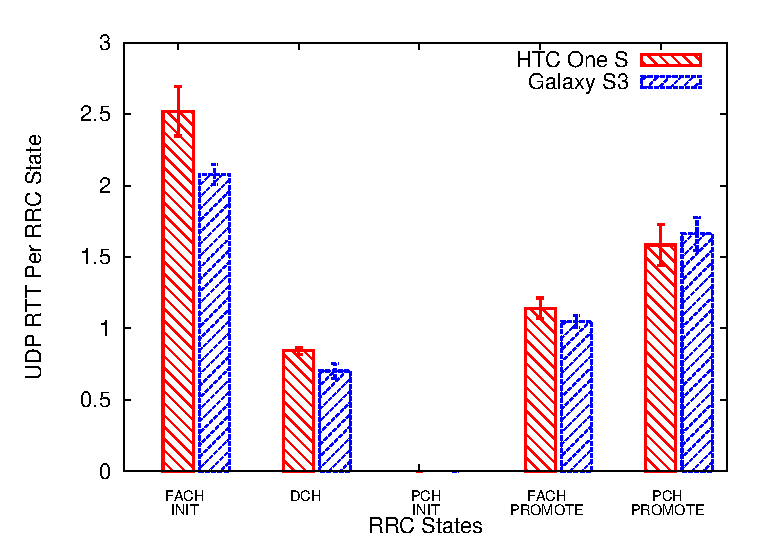
\includegraphics[width=0.5\textwidth]{figs/udp_rtt.eps}
%\ncaption{UDP RTT calculated from the QxDM log result}
%\label{fig:udp.rtt}
%\end{figure}

\subsection{Cross-Layer Mapping Algorithm}\label{sec:cross.layer.algo}

% Describe the mapping algorithm we use for cross-layer analysis
Correlating the transport layer packets with the RLC layer transmitted PDUs would allow us a transparent view of link layer behavior, especially RLC retransmissions.  One major limitation we need to address when using QxDM to analyze data is that packet logging is incomplete. Only the header and first byte of the data payload is logged for each RLC PDU. Furthermore, it is also possible for a small number of RLC PDUs to not be captured, leading to a sequence number gap. We created a mapping algorithm to address these limitations.

% The mapping algorithm here
The cross-layer mapping algorithm maps complete IP packets (known as SDUs, or \textit{Service Data Units}) to the corresponding fragmented RLC payload (or PDU).  PDUs have a fixed size which we denote as $S_{PDU}$.  The basic idea is that we find the first byte of the RLC PDU that matches the first byte of an SDU.  We then skip forward from that byte in the SDU by $S_{PDU}$, and check if that next byte matches the next RLC PDU.  As well, if the sequence number difference $D$ between two consecutive PDUs is greater than 1, then some RLC PDUs are missing from the QxDM trace.  In that case, we skip ahead by $S_{PDU} \times D$ instead.  We know our mapping is complete if every PDU's first byte maps to an SDU, with the SDU bytes being the appropriate distance apart and with the ordering of PDUs and SDUs being conserved.  Otherwise, no mapping was discovered.

%creates a mapping between complete IP packets (also known as SDUs, or \textit{Service Data Units}) and the corresponding fragmented RLC payloads (or the PDUs). The basic idea is that once we find one RLC PDU's first byte matching with the first byte of SDU, then we skip to the next byte at one PDU size away from SDU's first byte to check whether the next RLC PDU's first byte matches that byte. If the sequence number difference (\textbf{D}) between two consecutive RLC PDU is greater than 1, that implies the some RLC PDUs in between were not captured in QxDM. Then we skip the \textbf{D} times of PDU size bytes for SUD in the algorithm. If we map all every PDUs size of byte in SDU to a list of RLC PDU, then we successfully find a mapping; otherwise no mapping was discovered.
 % It is necessary to determine the end of the IP packet associated with each PDU as we iterate over the PDUs. Unfortunately, each PDU can contain either payload data from a single SDU, or from two SDUs.  If an SDU does not fill a PDU then par of the next SDU will be concatenated to fill the rest of the space~\cite{spec-3G-RLC}, to increase transmission efficiency. 
 \TReport{Algorithm~\ref{alg:cross.mapping} describes this mapping mechanism in detail.}
%If the cumulative mapped index equals the size of the SDU (or the length of IP packets), we have successfully found a mapping; otherwise no mapping was discovered.

%is essentially a map between the complete IP packets (known as SDU) and corresponding fragmented RLC payload data bytes (known as PDU). Due to the partial logged information in QxDM, only the first data byte is captured in the log. Thus, we have to skip over the rest of the PDU, and try to match for the first data byte in the next PDU. The problem at this point is to determine the end of IP packets while we iterate through the consecutive RLC PDUs. Since each PDU could either contain the payload data dedicated to a single SDU or belongs to two SDUs. If the reminder size of the SDU cannot fulfill the largest size of PDU, then RLC protocol will concatenate the part of the next SDU to fill the rest of space~\cite{spec-3G-RLC}. Ultimately, if the accumulative mapped index equals the size of SDU, we claim to find a mapping successfully; otherwise no mapping discovered. Algorithm ~\ref{alg:cross.mapping} states the detailed information of the mapping mechanism.

% the corner case of the mapping algorithm
% --- this is respesented by the ``factor" variable in the mapping algorithm.  %Sanae: this factor isn't actually mentioned any more.
However, this mapping mechanism cannot recover all packets in every case. In particular, this is true when missing PDUs are at the beginning or end of the mapped RLC list, but those cases occur rarely in the QxDM traces. We evaluate the accuracy of this improved mapping algorithm by observing the percentage of mapped IP packets in both the \emph{QxDM\_{}TCP\_{}Trace} and the \emph{QxDM\_{}TCP\_{}Trace}. We were able to correctly map 99.8\% of packets. 

%\mycomment{besides using mapping coverage as a metric for evaluation, what are other ways we can validate the correctness of the mapping? Answer: another way to validate the mapping is to map group of RLC PDU back to the TCP/UDP packets, but due to missed log information, we are not 100\% confidence in that direction.}

%There is a corner case in the mapping algorithm such that the QxDM cannot capture the some of the SDUs. Similar to TCP protocol, the sequence number in RLC PDUs could uniquely distinguish between every PDUs. If there are some missed PDUs, then we cannot map the first byte data for every PDU size. In that case, we could even skip over the missed PDUs and add up multiple of PDU size to hunt for a match, which is represented as "factor" variable in the mapping algorithm. However, the aggressive leap mapping mechanism cannot fully recover the corner case, especially when the missed PDUs were either the beginning or the end part of the mapped RLC list. We evaluate the improved mapping algorithm by checking the percentage of mapped IP packets in all the traces of control experiments, and the average mapping ratio is \textit{99.8\%}.

% algorithm detail
\begin{TReports} 

\begin{algorithm}[t!]
\begin{algorithmic}[width=0.5\textwidth]
\STATE {\textit{\textbf{Function} Cross-Layer-Mapping(SDU, PDU\_{}LIST):}}
\STATE {// point to the current mapped PDU in \textit{PDU\_{}LIST}}
\STATE {Initialize \textit{PDU\_{}INDEX} as $0$}
\STATE {// point to the current mapped byte in SDU)}
\STATE {Initialize \textit{SDU\_{}MAPPED\_{}INDEX} as $0$}
\STATE {Initialize \textit{MAPPED\_{}PDU\_{}LIST} as empty list}
\WHILE {PDU\_{}INDEX is less than length of PDU\_{}list}
\WHILE {\textit{SDU\_{}MAPPED\_{}INDEX} $<$ SDU size}
\IF {\textit{SDU[SDU\_{}MAPPED\_{}INDEX]} equals to \textit{CUR\_{}PDU}}
	\STATE {// Success to map current byte}
	\STATE {Append \textit{CUR\_{}PDU} to \textit{MAPPED\_{}PDU\_{}LIST}}
	\STATE {\textit{CUR\_{}PDU} = \textit{PDU\_{}LIST[PDU\_{}INDEX]}}
	\STATE {$factor$ is seq\_{}num between \textit{CUR\_{}PDU} and \textit{LAST\_{}PDU}}
	\STATE {Set \textit{LAST\_{}PDU} as \textit{CUR\_{}PDU}}
	\IF {\textit{cur\_{}PDU} has LI field in header}
		\STATE {Increase \textit{SDU\_{}MAPPED\_{}INDEX} by the value of LI field}
	\ELSE
    		\STATE {Increase \textit{SDU\_{}MAPPED\_{}INDEX} by the size of \textit{CUR\_{}PDU} multiples $factor$}
    	\ENDIF
    	\IF {\textit{CUR\_{}PDU}'s HE field indicate last PDU}
    		\STATE {Break}
    \ENDIF
\ELSE
	\STATE {// fail to map the current byte}
	\STATE {Reset \textit{MAPPED\_{}PDU\_{}LIST} as empty list}
	\STATE {Reset \textit{SDU\_{}MAPPED\_{}INDEX} as $0$}
	\STATE {Break}
\ENDIF
\STATE {Increase \textit{PDU\_{}INDEX} by $1$}
\ENDWHILE
\IF {\textit{SDU\_{}MAPPED\_{}INDEX} equals to SDU size}
	\STATE {// Success to find a mapping!}
	\RETURN {\textit{MAPPED\_{}PDU\_{}LIST}}
\ENDIF
\ENDWHILE
\RETURN {\textit{NOT FOUND}}
\end{algorithmic}
\caption{Map the SDU to the corresponding PDU list}
\label{alg:cross.mapping}
\end{algorithm}

\end{TReports} 

\subsection{RLC Retransmission Calculation}\label{sec:rlc.retx.cal}

The RLC layer includes a retransmission mechanism to improve the reliability of transmissions over the lossy data transmission channel.  However, this may not eliminate unnecessary retransmissions,  as it acts independent of upper layers. This is especially problematic for TCP retransmission timeouts. We describe in this section how we determine when RLC retransmission has occurred from the QxDM logs.

%The RLC layer retransmission is a protection mechanism that maximize the reliability over a loss data transmission channel. However, it also causes the delays due to duplicate transmissions without noticing the upper layers. To assist further identifying the root cause of the latency, we first introduce how we calculate the RLC retransmission from the QxDM logs.

% how to calculate the RLC retransmission
Each RLC sequence number uniquely identifies each RLC PDU, so we can determine RLC retransmissions based on duplicate sequence numbers.  One complication is that sequence numbers wrap around every 4096 PDUs.  To avoid over-counting duplicate sequence numbers from a different cycle, a window size of 512 PDUs is set to count how often sequence numbers reappear. The number of RLC retransmissions is the cumulative count of the repeated sequence number for a given list of RLC PDUs~\cite{spec-3G-RLC}.

% RLC retransmission Ratio calculation
The RLC retransmission ratio measures the relative frequency of RLC retransmissions over a range of time as defined in Table ~\ref{tab:terminology}. First, we describe how to determine the retransmission ratio for a RRC state. The RRC state for each RLC PDU is determined by backtracking to the most recent RRC state QxDM log entry. RLC-layer retransmitted PDU counts are broken down based on the RRC states where they were transmitted. By dividing the total number of retransmitted PDUs by the total number of PDUs in each RRC state, the retransmission ratio can be calculated. We also calculate the RLC layer retransmission ratio for specific inter-packet times (as described in \S\ref{sec:methodology}) by  counting retransmissions over a certain inter-packet time transmission period.

%The sequence number of the RLC PDU will uniquely identify each RLC packet. Therefore, we determine the RLC retransmission based on the duplicate of sequence numbers. Since the size of RLC PDU is only 42 bytes and is very limited, if the RLC keeps an effective throughput, it has to reduce the number of bits in the header to hold the sequence number. Therefore, the sequence number only consumes 12 bits (range of 0-4095) in the current RLC protocol~\cite{spec-3G-RLC}. As a result, sequence number is circularly reused every 4096 PDUs, and it is always increasing. To avoid over-count the duplicate sequence number in different cycle, we hard set a smaller window size of 512 to count the reappearing sequence number within that range. We determine the RRC state for each RLC PDU by backtracking to most recent RRC state log entry, and fetch the RRC state based on that log content. We break down RLC retransmitted PDUs based on their RRC states when they were transmitted, and we calculate the retransmission ratio through dividing total number of retransmitted PDUs per RRC state by the total number of PDUs in that RRC state.
